\subsection{Gap mínimo para chute à gol}
Somente o peso do parâmetro que permite chute à gol
foi alterado para $5$. Os resultados no planejamento são
apresentados na figura~\ref{fig:min_gap_5}.

\begin{figure}[H]
  \centering
  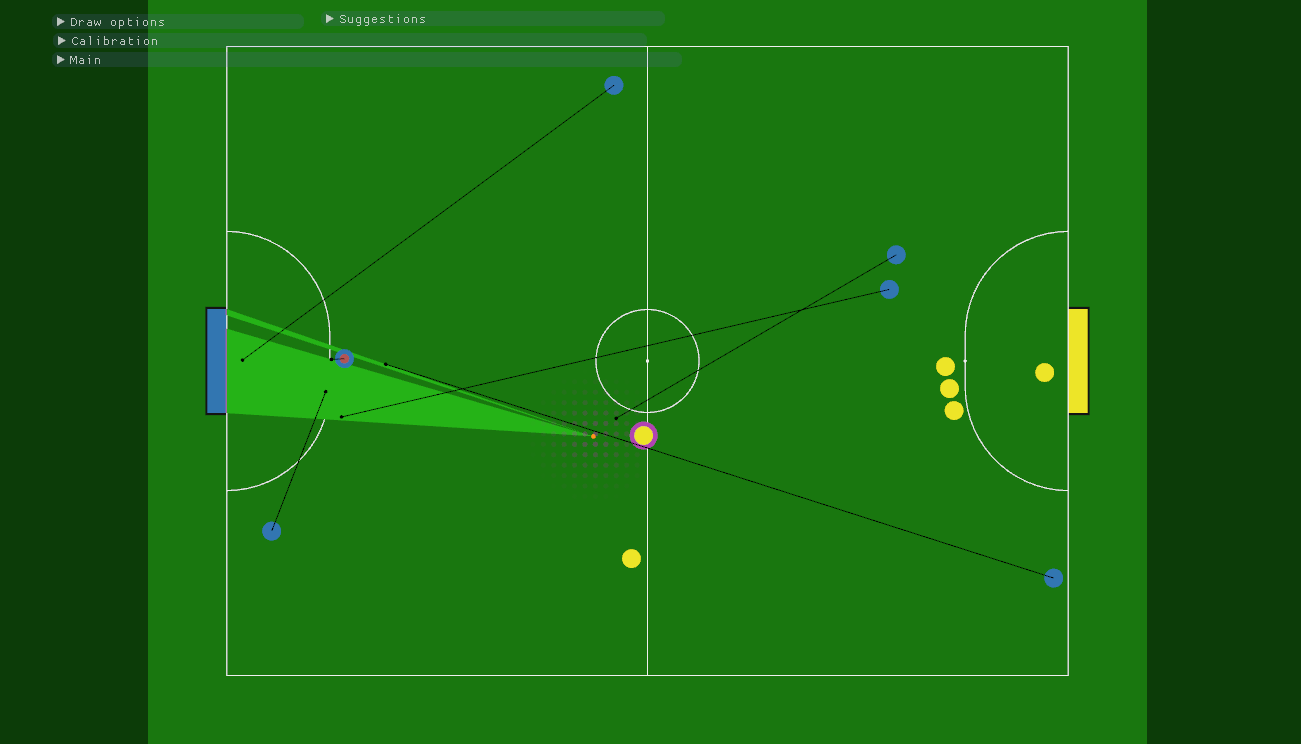
\includegraphics[width= 0.8\linewidth]{result/min_gap_def_5}
  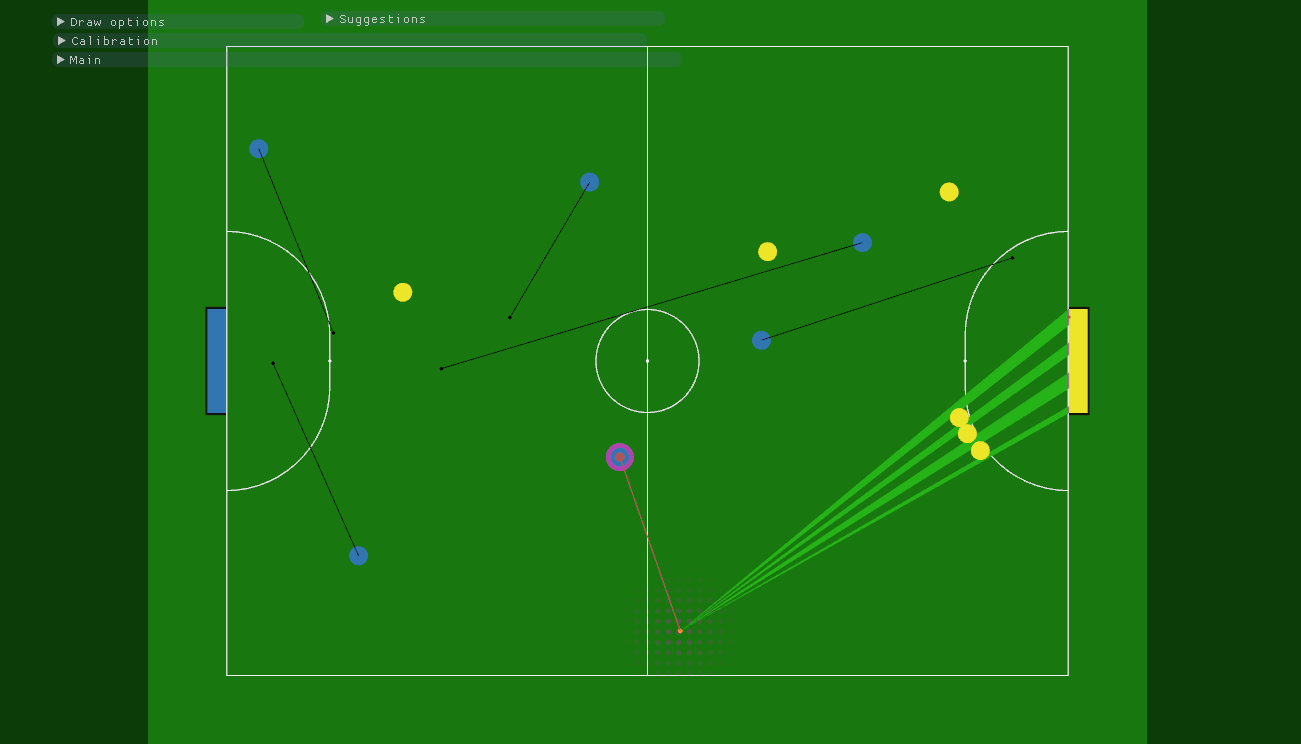
\includegraphics[width= 0.8\linewidth]{result/min_gap_atq_5}
  \caption{Planejamento com os parâmetros iniciais e com o gap
           mínimo para chute alterado para $5$.
           No ataque (acima) e na defesa (abaixo)}\label{fig:min_gap_5}
\end{figure}
